\documentclass{article}
\usepackage[margin=1.5in]{geometry}

%%%% PACKAGES TO USE
\usepackage[utf8]{inputenc} % allow utf-8 input
\usepackage[T1]{fontenc}    % use 8-bit T1 fonts
\usepackage{hyperref}       % hyperlinks
\usepackage{url}            % simple URL typesetting
\usepackage{booktabs}       % professional-quality tables
\usepackage{amsfonts}       % blackboard math symbols
\usepackage{nicefrac}       % compact symbols for 1/2, etc.
\usepackage{microtype}      % microtypography

% Math related
\usepackage{amsmath}
% Indicator
%\usepackage{bbm} %uses Type3
\usepackage{dsfont} %works with Type1
% Figures and subfigures
\usepackage{graphicx}
\usepackage{caption}
\usepackage{subcaption}
\usepackage{float} %Stay where told
% Tables
\usepackage{booktabs} % for professional tables
\usepackage{multirow} % to be able to have multiple row expanding cell
\usepackage[table]{xcolor}
% Reference column balancing
\usepackage{flushend}
% Algorithms
\usepackage{algorithm}
\usepackage{algorithmic}
% To draw graphs
\usepackage{tikz}
\usetikzlibrary{bayesnet} % Library for bayesian networks

% Bibliography
\usepackage[round,numbers,sort]{natbib}

%%%% DEFINITIONS-MACROS
% Real line
\def \Real{{\mathbb R}} 
\def \Natural{{\mathbb N}} 
%Expected value
\newcommand{\eValue}[1]{\mathbb{E}\left\{ #1 \right\}}
% My small matrix
\newcommand{\mySmallMatrix}[1]{\left(\begin{smallmatrix} #1 \end{smallmatrix}\right)}
%Determinant
\newcommand{\mydet}[1]{\left| #1 \right|}
\newcommand{\HH}{\mathcal{H}}

% Abbreviations
\newcommand{\iid}{i.i.d. }
\newcommand{\ie}{i.e., }
\newcommand{\Ie}{I.e., }
\newcommand{\eg}{e.g., }
\newcommand{\Eg}{E.g., }
\newcommand{\etAl}{et al.\xspace}

%Distributions
\newcommand{\N}[1]{\mathcal{N}\left( #1\right)}
\newcommand{\MN}[1]{\mathcal{MN}\left( #1\right)}
\newcommand{\T}[1]{\mathcal{T}\left( #1\right)}
\newcommand{\MT}[1]{\mathcal{MT}\left( #1\right)}
\newcommand{\Dir}[1]{{\rm Dir\left( #1\right)}}
\newcommand{\Mult}[1]{{\rm Mult}\left( #1\right)}
\newcommand{\Cat}[1]{{\rm Cat}\left( #1\right)}
\newcommand{\Bin}[1]{{\rm Bin}\left( #1\right)}
\newcommand{\IG}[1]{{\rm IG}\left( #1\right)}
\newcommand{\NIG}[1]{{\rm NIG}\left( #1\right)}
\newcommand{\NIX}[1]{{\rm NIX}\left( #1\right)}
\newcommand{\IW}[1]{{\rm IW}\left( #1\right)}
\newcommand{\NIW}[1]{{\rm NIW}\left( #1\right)}
\newcommand{\Beta}[1]{{\rm Beta}\left( #1\right)}
\newcommand{\Ber}[1]{{\rm Ber}\left( #1\right)}
\newcommand{\U}[1]{\mathcal{U}\left( #1\right)}

%Others
\newcommand{\eqd}{\stackrel{d}{=}} % equal in distribution/law/measure
\newcommand{\deq}{:=} % Define equality
\newcommand{\abs}[1]{|{#1}|}
\newcommand{\argmax}{\mathop{\mathrm{argmax}}}
\newcommand{\argmin}{\mathop{\mathrm{argmin}}}
\newcommand{\var}{\textrm{Var}}
\newcommand{\cov}{\textrm{Cov}}
\newcommand{\Var}{\mathbb{V}\mathrm{ar}}
\newcommand{\Cov}{\mathrm{Cov}}
\newcommand{\tr}[1]{\mathrm{tr}\left\{ #1 \right\}} % trace
\newcommand{\diag}{\mathrm{diag}}
\newcommand{\ind}[1]{\mathds{1}_{#1}} % Indicator function
\newcommand{\kl}{\textrm{KL}}
\newcommand{\indep}{{\;\bot\!\!\!\!\!\!\bot\;}}
\newcommand{\eps}{\varepsilon}

% Whether to add appendix or not
\def\addappendix{}
%%%%%%%% end iurteaga %%%%%%%% 

\title{Nonparametric Gaussian mixture models for the multi-armed contextual bandit}

\author{ I\~{n}igo Urteaga and Chris H.~Wiggins\\
	{\sf \{inigo.urteaga, chris.wiggins\}@columbia.edu} \\\\
	Department of	Applied Physics and Applied Mathematics\\
	Data Science Institute\\
	Columbia University\\
	New York City, NY 10027
}

\begin{document}

\maketitle

\begin{abstract}
The multi-armed bandit is a sequential allocation task where an agent must learn a policy that maximizes long term payoff, where only the reward of the played arm is observed at each iteration. In the stochastic setting, the reward for each action is generated from an unknown distribution, which depends on a given `context', available at each interaction with the world. Thompson sampling is a generative, interpretable multi-armed bandit algorithm that has been shown both to perform well in practice, and to enjoy optimality properties for certain reward functions. Nevertheless, Thompson sampling requires sampling from parameter posteriors and calculation of expected rewards, which are possible for a very limited choice of distributions. We here extend Thompson sampling to more complex scenarios by adopting a very flexible set of reward distributions: nonparametric Gaussian mixture models. The generative process of Bayesian nonparametric mixtures naturally aligns with the Bayesian modeling of multi-armed bandits. This allows for the implementation of an efficient and flexible Thompson sampling algorithm: the nonparametric model autonomously determines its complexity in an online fashion, as it observes new rewards for the played arms. We show how the proposed method sequentially learns the nonparametric mixture model that best approximates the true underlying reward distribution. Our contribution is valuable for practical scenarios, as it avoids stringent model specifications, and yet attains reduced regret.
\end{abstract}

\section{Introduction}
\label{sec:introduction}

Recent advances in reinforcement learning \cite{j-Gosavi2009} have sparked renewed interest in sequential decision making. The aim of sequential decision making is to optimize interactions with the world (exploit) while simultaneously learning how the world operates (explore). Its origins can be traced back to the beginning of the past century, with important contributions within the field of statistics by \citet{j-Thompson1935} and later \citet{j-Robbins1952}. The multi-armed bandit (MAB) problem is a natural abstraction for a wide variety of real-world challenges that require learning while simultaneously maximizing rewards.

The name ``bandit'' finds its origin in the playing strategy one must devise when facing a row of slot machines. The contextual setting, where at each interaction with the world side information (known as `context') is available, is a natural extension of the bandit problem. Recently, a renaissance of the study of MAB problems has flourished \cite{j-Scott2010,j-Agrawal2011,ip-Maillard2011}. The performance of algorithms for contextual bandits with linear payoffs \cite{j-Rusmevichientong2010, ip-Chu2011} has been widely studied in the last decade \cite{ic-Langford2008,j-Cesa-Bianchi2011,ic-Abbasi-Yadkori2011}. Furthermore, it has attracted interest from industry, due to its impact in digital advertising and products \cite{j-Li2010, ic-Chapelle2011}. 

Thompson Sampling \cite{j-Thompson1933, j-Russo2018} and its generalization known as posterior sampling, provide an elegant approach that tackles the exploration-exploitation dilemma. It updates a posterior over expected rewards, and chooses actions based on the probability that they are optimal. It has been empirically and theoretically proven to perform competitively for many MAB models \cite{ic-Chapelle2011,j-Scott2015,j-Agrawal2012,j-Agrawal2012a,ic-Korda2013,j-Russo2014,j-Russo2016}. Besides, its applicability to the more general reinforcement learning setting of Markov Decision Processes \cite{j-Burnetas1997} has recently tracked momentum \cite{ip-Gopalan2015,ic-Ouyang2017}.

Thompson sampling and the Bayesian modeling of the MAB problem facilitate not only generative and interpretable modeling, but sequential and batch processing algorithms as well. Within this framework, one only requires access to posterior samples of the model. Unfortunately, maintaining such a posterior is intractable for distributions not in the exponential family \cite{ic-Korda2013}. As such, developing practical MAB methods to balance exploration and exploitation in complex domains remains largely unsolved.

In an effort to extend Thompson sampling to more complex scenarios, researchers have considered other flexible reward functions and Bayesian inference. 
For example, recent approaches have embraced approximate Bayesian neural networks for Thompson Sampling. Neural networks have proven to be powerful function approximators, and approximate Bayesian inference provides posterior uncertainty estimates. To that end, variational methods, stochastic mini-batches, and Monte Carlo techniques have been studied for uncertainty estimation of posteriors \cite{ip-Blundell2015, ic-Kingma2015, j-Lipton2016, ic-Osband2016, ip-Li2016}. In a recent benchmark of such techniques \cite{ip-Riquelme2018}, it was reported that even if successful in the supervised learning setting, they under-perform in the MAB scenario. In particular, \citet{ip-Riquelme2018} emphasize the issue of adapting the slow convergence uncertainty estimates of neural net based methods to the bandit setting.

In parallel, others have focused on extending Thompson sampling by targeting alternative classes of reward functions. Some have focused on approximating the unknown bandit reward functions with Gaussian mixture models \cite{ip-Urteaga2018}, while others have assumed a Gaussian process reward distribution \cite{ip-Srinivas2010,ip-Gruenewaelder2010,ic-Krause2011}. The latter are powerful nonparametric methods for modeling distributions over non-linear continuous functions \cite{b-Rasmussen2005}. Unfortunately, standard Gaussian processes are computationally demanding, as they scale cubically in the number of observations, limiting their applicability to small datasets and the online setting (even if advancements such as pseudo-observations \cite{ic-Snelson2006} or variational inference \cite{ip-Titsias2009} have been proposed to mitigate these shortcomings).

In this paper, we combine the large hypothesis space of mixture models --- which can approximate any continuous reward distribution --- with the flexibility of Bayesian nonparametrics \cite{j-Gershman2012}. In many contexts, a countably infinite mixture is a very realistic model to assume, and has been shown to succeed in modeling a diversity of phenomena. Within the Bayesian framework, one uses prior distributions over the mixing proportions, such as Dirichlet or Pitman-Yor processes \cite{j-Teh2010}, which allow for inference of the appropriate complexity of a model from observed data. These models describe mixtures in which one not only does not explicitly specify the number of mixtures, but allows the possibility of an unbounded number of mixtures. Bayesian nonparametrics support a wide class of models, yet have analytically tractable inference and online update rules.

Our contribution here is on exploiting Bayesian nonparametric mixture models for Thompson sampling to perform MAB optimization. 
This provides a new flexible framework for solving a rich class of MAB problems. We model the complex mapping between the observed rewards and the unknown parameters of the generating process with nonparametric Gaussian mixture models. For learning such a nonparametric distribution within the contextual multi-armed bandit setting, we leverage the advances in Markov Chain Monte Carlo methods for Bayesian nonparametric models \cite{j-Neal2000}.

Mixtures of distributions provide a powerful approach for nonparametric density estimation, and the generative interpretation of Bayesian nonparametric models corresponds to the sequential nature of the MAB problem as well. The proposed method learns the nonparametric mixture model that best approximates the true underlying reward distribution, adjusting its complexity as it sequentially observes additional data. To the best of our knowledge, no other work uses Bayesian nonparametric mixture models to address the contextual MAB.

We formally introduce the MAB problem and the Bayesian nonparametric framework in Section~\ref{sec:background}, before providing the description of the proposed nonparametric Thompson sampling in Section~\ref{sec:proposed_method}. We evaluate its performance in Section~\ref{sec:evaluation}, and suggest generalizations in Section~\ref{sec:conclusion}.

\section{Background}
\label{sec:background}

\subsection{Multi-armed bandits}
\label{ssec:background_mab}
A multi-armed bandit is a real time sequential decision process in which, at each iteration, an agent is asked to select an action according to a policy which maximizes the accumulated rewards over time, balancing exploitation and exploration. In the contextual case, one must decide which arm $a\in\{0,\cdots,A-1\}$ to play next (\ie pick $a_{t+1}$), based on the available context, e.g.,  $x_{t+1}\in\Real^{d}$. At every iteration  $t$, the observed reward $y_t$ is independently drawn from the unknown reward distribution corresponding to the played arm, conditioned on the context and parameterized by unknown $\theta$; \ie $y_t\sim p_{a}(y|x_t,\theta)$. Due to the stochastic nature of the bandit, one summarizes each arm's reward via its conditional expectation for that context $\mu_{a}(x,\theta)=\mathbb{E}_{a}\{y|x,\theta\}$.

When the properties of the arms (\ie the parameters $\theta$) are known, one can readily determine the optimal selection policy as soon as the context is given, \ie
\begin{equation}
a^*(x,\theta)=\argmax_{a}\mu_{a}(x,\theta) \; .
\end{equation}
The challenge in the contextual MAB problem is not knowing the true reward parameters $\theta$ or, more generally, the lack of knowledge about the reward-generating model. Thus, one needs to simultaneously (1) learn the properties of the reward distribution and (2), decide which action to take sequentially. The next arm to play is chosen based upon the history observed, with the goal of maximizing the expected (cumulative) reward. Previous history contains the set of given contexts, played arms, and observed rewards up to time $t$, denoted as $\mathcal{H}_{1:t}=\left\{x_{1:t}, a_{1:t}, y_{1:t}\right\}$, with $x_{1:t} \equiv (x_1, \cdots , x_t)$, $a_{1:t} \equiv (a_1, \cdots , a_t)$ and $y_{1:t} \equiv (y_1, \cdots , y_t)$. 

Among the many alternatives to address this class of problems, Thompson sampling is particularly appealing, due to its generative formulation and its connection with Bayesian modeling. Furthermore, it has been shown to perform empirically well and has sound theoretical bounds, for both contextual and context-free problems \cite{ic-Chapelle2011,j-Agrawal2012,j-Agrawal2012a,ic-Korda2013,j-Russo2014,j-Russo2016}.

Thompson sampling chooses what arm to play in proportion to its probability of being optimal, \ie
\begin{equation}
a_{t+1} \sim \mathrm{Pr}\left[a=a_{t+1}^*|x_{t+1}, \theta, \mathcal{H}_{1:t}\right] \;,
\end{equation} 
where $a_{t+1}^*$ is the optimal arm given the true parameters and the observed context, \ie $a_{t+1}^*=\argmax_{a}\mu_{a}(x_{t+1},\theta)$. If the parameters of the model are known, the above expression becomes deterministic, as one always picks the arm with the maximum expected reward
\begin{equation}
\mathrm{Pr}\left[a=a_{t+1}^*|x_{t+1}, \theta, \mathcal{H}_{1:t} \right] = \mathrm{Pr}\left[a=a_{t+1}^*|x_{t+1}, \theta \right] = I_a(x_{t+1},\theta) \;,
\label{eq:theta_known_pr_arm_optimal}
\end{equation}
where $I_a(\cdot)$ denotes the indicator function
\begin{equation}
I_a(x,\theta) = \begin{cases}
1, \; \mu_{a}(x,\theta)=\max\{\mu_1(x,\theta), \cdots, \mu_A(x,\theta)\} \;, \\
0, \; \text{otherwise} \;.
\end{cases}
\end{equation}

When the parameters of the model are unknown, one needs to explore ways of computing the probability of each arm being optimal. In a Bayesian setting, the parameters are modeled as random variables with priors. Specifically, one marginalizes over the posterior probability distribution of the parameters, after observing rewards and actions up to time instant $t$, \ie
\begin{equation}
\begin{split}
\mathrm{Pr}\left[a=a_{t+1}^* \big| \mathcal{H}_{1:t}\right] & = \int p(a=a^*|x_{t+1}, \theta, \mathcal{H}_{1:t}) p(\theta|\mathcal{H}_{1:t}) \mathrm{d}\theta =\int I_a(x_{t+1}, \theta) p(\theta|\mathcal{H}_{1:t}) \mathrm{d}\theta \; .
\end{split}
\label{eq:theta_unknown_pr_arm_optimal}
\end{equation}

The above integral can not be solved exactly, even when the parameter posterior update is analytically tractable. Therefore, when reward distributions that are not within the exponential family are considered, one must resort to approximations of the posterior. In the following, we propose nonparametric mixture models as tractable yet performant reward distributions for the MAB.

\subsection{Bayesian nonparametric mixture models}
\label{ssec:background_nonparametric_mixture_model}

Bayesian nonparametric models provide a powerful density estimation framework that adjust model complexity in response to the data observed. The combination of mixture models with Bayesian nonparametrics embodies a large hypothesis space, which can arbitrarily approximate continuous reward distributions. Bayesian nonparametric mixture models describe countably infinite mixture distributions, which are very flexible assumptions suited for many practical settings. We refer to \cite{j-Gershman2012} for a detailed review of standard nonparametric models and how they can be used in practice.

A variety of Bayesian nonparametric alternatives have been studied in literature. We here focus on the Pitman-Yor model, which is a stochastic process whose sample path is a probability distribution. It is a generalization of Bayesian nonparametric models from where a drawn random sample is an infinite discrete probability distribution. In the following, we succinctly summarize the generative process and the basics for its inference.

A Pitman-Yor mixture model \cite{j-Teh2010}, with a discount parameter $0 \leq d < 1$ and a concentration parameter $\gamma > -d$, is described by the following generative process:
\begin{enumerate}
	\item Mixture parameters are drawn from the Pitman-Yor process, \ie $\theta_n \sim G$, where $G=PY(d, \gamma, G_0)$. Equivalently, the process can be described as 
	\begin{equation}
	\theta_{n+1}|\theta_{1:n}, d, \gamma, G_0 \sim \sum_{k=1}^{K} \frac{n_k-d}{n+\gamma}\delta_{\theta_k} + \frac{\gamma+Kd}{n+\gamma}G_0 \; ,
	\label{eq:pitman_yor_mixture}
	\end{equation}
	where $n$ refers to all the available observations, and $n_k$ to the number of observations assigned to mixture $k$.
	\item The observation is drawn from the emission distribution parameterized by its corresponding parameters, \ie $y_{n+1} \sim f(y|\theta_{n+1})$.
\end{enumerate}

For parametric measures, we write $G_0(\theta)=G(\theta|\Theta_0)$ and $G_n(\theta)=G(\theta|\Theta_n)$, where $\Theta_0$ are the prior hyperparameters of the emission distribution, and $\Theta_n$ are the posterior parameters after $n$ observations.

We note that the Dirichlet process can be readily obtained from Eqn.~\eqref{eq:pitman_yor_mixture} by using $d=0$. The discount parameter gives the Pitman-Yor process more flexibility over tail behavior (the Dirichlet process has exponential tails, whereas the Pitman-Yor can have power-law tails).

For analysis and inference of these models, one incorporates auxiliary mixture variables $z_n$. These are categorical variables, where $z_{n}=k$, if observation $y_n$ is drawn from mixture $k$. The joint posterior of these assignments follows, for $d=0$,
\begin{equation}
p(z_{1:n}|\gamma) = \prod_{i=1}^n p(z_i|z_{1:n-1},\gamma) = \frac{\gamma^K \prod_{k=1}^K(n_k-1)!}{\prod_{i=1}^n (i-1+\gamma)} = \frac{\Gamma(\gamma)}{\Gamma(\gamma+n)} \gamma^K \prod_{k=1}^K\Gamma(n_k) \; ,
\end{equation}
where $n_k$ indicates the number of observations drawn from mixture $k$ and $n=\sum_{k=1}^Kn_k$. The full joint likelihood of assignments and observations is 
\begin{equation}
p(y_{1:n},z_{1:n}|\gamma, \Theta) = p(y_{1:n}|z_{1:n}, \Theta) p(z_{1:n}|\gamma) = p(y_{1:n}|z_{1:n}, \Theta) \left( \frac{\gamma^K \prod_{k=1}^K(n_k-1)!}{\prod_{i=1}^n (i-1+\gamma)} \right) \; .
\end{equation}

For inference of the above model given observations $y_{1:n}$, one can derive a Gibbs sampler that iterates between mixture assignment sampling and posterior updates of the emission distribution parameters (\citet{j-Teh2010} provide a detailed explanation of the procedure).

The conditional distributions of observation assignments $z_n$ to already drawn mixtures $k\in\{1, \cdots, K\}$, and a new unseen mixture $k_{new}$ are
\begin{equation}
\begin{cases}
p(z_{n+1}=k|y_{n+1},y_{1:n},z_{1:n}, \gamma, G_0) \propto \frac{n_k-d}{n+\gamma} \int_{\theta} f(y_{n+1}|\theta_{n+1}) G_n(\theta) \mathrm{d}\theta \; ,\\
p(z_{n+1}=k_{new}|y_{n+1},y_{1:n},z_{1:n}, \gamma, G_0) \propto \frac{\gamma+K d}{n+\gamma} \int_{\theta} f(y_{n+1}|\theta_{n+1}) G_0(\theta) \mathrm{d} \theta \; .\\
\end{cases}
\label{eq:gibbs_mixture_assignment}
\end{equation}

Given these mixture assignments, one updates the parameter posteriors conditioned on $z_{1:n}$ and observations $y_{1:n}$, based on the specific choices of emission distribution and priors: $G_n(\theta)=G(\theta|y_{1:n}, z_{1:n},\Theta_0)$. These also determine the computation of the predictive distribution $f(y|\Theta)= \int_{\theta} f(y|\theta) G(\theta|\Theta) \mathrm{d} \theta$ for solving Eqn.~\eqref{eq:gibbs_mixture_assignment}. For analytical convenience, one usually resorts to emission distributions with their conjugate priors.

\section{Proposed method}
\label{sec:proposed_method}

We now describe how to combine Bayesian nonparametric mixture models with Thompson sampling for the MAB setting. The graphical model of the Bayesian nonparametric MAB is rendered in Fig. \ref{fig:pgm_nonparametric_bandit}. We consider a completely independent set of nonparametric mixture models $G_{a,0}$ per arm, with their own hyperparameters $d_a$ and $\gamma_a$.

% Nonparametric bandit graphical model
\begin{figure}[!h]
	\begin{center}
		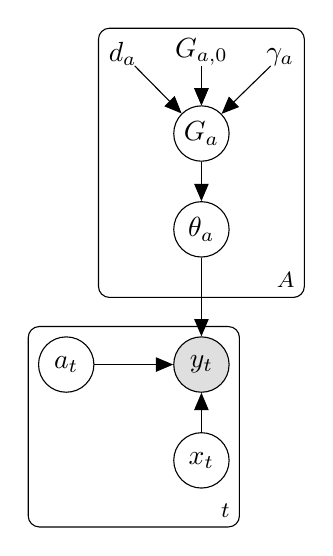
\begin{tikzpicture}
	% Nodes
	% Return y
	\node[obs] (y-t) {$y_{t}$};
	% Nonparametric parameters
	\node[latent, above=1.0 of y-t, xshift=0cm] (theta-a) {$\theta_{a}$};
	% Nonparametric distribution
	\node[latent, above=0.5 of theta-a, xshift=0cm] (G-a) {$G_{a}$};
	% Action a
	\node[latent, left=1 of y-t] (a-t) {$a_t$};
	% Context x
	\node[latent, below=0.5 of y-t]  (x-t) {$x_t$};
	
	% Hyperparameters
	\node[const, above=0.5 of G-a, xshift=-1.0cm] (d-a) {$d_{a}$} ;
	\node[const, above=0.5 of G-a, xshift=1.0cm] (gamma-a) {$\gamma_{a}$} ;
	\node[const, above=0.5 of G-a, xshift=0.0cm]  (G-a0) {$G_{a,0}$} ;
	
	% Edges
	% Hyperparameters to distribution
	\edge {gamma-a,G-a0} {G-a} ;
	\edge {d-a,G-a0} {G-a} ;
	% Connect distribution to parameters
	\edge {G-a} {theta-a} ;
	% Connect parameters, context and arm to observation
	\edge {theta-a,x-t,a-t} {y-t} ;
	
	% Plates
	% Over time
	\plate {t} {(a-t)(x-t)(y-t)} {$t$} ;
	% Over each arm
	\plate {a}{
		(d-a)(gamma-a)(G-a0) % hyperparameters
		(G-a) % distribution
		(theta-a) % parameters
	} {$A$} ;
\end{tikzpicture}
	\end{center}
	\caption{Graphical model of the nonparametric mixture bandit distribution.}
	\label{fig:pgm_nonparametric_bandit}
\end{figure}

As shown in Fig. \ref{fig:pgm_nonparametric_bandit}, we assume complete independence of per-arm reward distributions, \ie each arm of the bandit is allowed to follow a different family of distributions. We consider this setting to be a very powerful extension of the MAB problem, which has not attracted much interest so far.

An alternative would be to consider a hierarchical-nonparametric model \cite{j-Teh2006,j-Teh2010}, where all arms are assumed to obey the same family of distributions, but only their mixture proportions are allowed to vary across arms. The main advantage of this alternative is that one would learn parameter posteriors from rewards of all played arms, with the disadvantage of all arms being limited to the same family of reward distributions. We illustrate this alternative hierarchical nonparametric MAB, and provide details of the model and its inference, in \ifx\addappendix\undefined the supplementary material\else \autoref{asec:nonparametric_hierarchical_mixture_model}\fi.

In order to approximate any continuous reward distribution, we study nonparametric Gaussian mixtures as a flexible formulation for modeling complex MAB reward densities.

We focus on context-conditional Gaussian emission distributions $y\sim \N{y|x^\top w_{a,k}, \sigma_{a,k}^2}$, which are parameterized per-arm and per-mixture; \ie $\theta_{a,k}=\{w_{a,k}, \sigma_{a,k}^2 \}$. The conjugate prior for such emission distribution is a Normal-inverse Gamma, with hyperparameters $\Theta_{a,0}=\{u_{a,0}, V_{a,0},\alpha_{a,0}, \beta_{a,0}\}$, \ie
\begin{equation}
G_{a,0}(\theta_a)=\NIG{w_a, \sigma_a^2 |u_{a,0}, V_{a,0},\alpha_{a,0}, \beta_{a,0}} = \N{w_a|u_{a,0}, \sigma_a^2 V_{a,0}} \Gamma^{-1}(\sigma_a^2|\alpha_{a,0}, \beta_{a,0}) \;.
\end{equation}

After observing rewards $y_{1:n}$, and conditioned on assignments $z_{1:n}$, the posteriors of the parameters per arm and mixture $\theta_{a,k}$ also follow a Normal-inverse Gamma distribution.

\clearpage
The updated hyperparameters of such posterior depend on the number $n_{a,k}$ of rewards observed after playing arm $a$ that are assigned to mixture $k$:
\begin{equation}
\begin{split}
G_{a,n_{a,k}}(\theta_{a,k})&=\NIG{w_{a,k}, \sigma_{a,k}^2 |u_{a,k,n_{a,k}}, V_{a,k,n_{a,k}},\alpha_{a,k,n_{a,k}}, \beta_{a,k,n_{a,k}}} \;,\\
\Theta_{a,k,n_{a,k}}= &\begin{cases}
V_{a,k,n_{a,k}}^{-1} = x_{1:n} R_{a,k} x_{1:n}^\top + V_{a,0}^{-1} \;,\\
u_{a,k,n_{a,k}}= V_{a,k,n_{a,k}} \left( x_{1:n} R_{a,k} y_{1:n} + V_{a,0}^{-1} u_{a,0}\right) \;, \\
\alpha_{a,k,n_{a,k}} = \alpha_{a,0} + \frac{1}{2} \tr{R_{a,k}} \;, \\
\beta_{a,k,n_{a,k}} = \beta_{a,0} + \frac{1}{2}\left(y_{1:n}^\top R_{a,k}y_{1:n} \right) \\
\hspace*{2cm}+ \frac{1}{2}\left( u_{a,0}^\top V_{a,0}^{-1} u_{a,0} - u_{a,k,n_{a,k}}^\top V_{a,k,n_{a,k}}^{-1} u_{a,k,n_{a,k}} \right) \; ,
\end{cases}
\end{split}
\label{eq:posterior_hyperparameters}
\end{equation}
where $R_{a,k}\in\Real^{n_a\times n_a}$ is a sparse diagonal matrix with elements $\left[R_{a,k}\right]_{n,n^\prime}=\mathds{1}[a_n=a,z_n=k]$, and $n_{a}$ the number of rewards observed after playing arm $a$.

Finally, the predictive emission distribution after marginalization of the parameters $\theta_{a,k}$, needed for solving Eqn.~\eqref{eq:gibbs_mixture_assignment}, follows a conditional Student-t distribution
\begin{equation}
\begin{split}
f_{a,k}(y|x) & = \T{y|\nu_{a,k,y}, m_{a,k,y}, r_{a,k,y}} \\
	&= \frac{\Gamma\left(\frac{\nu_{a,k,y}+1}{2}\right)}{\sqrt{\nu_{a,k,y} \pi} \cdot r_{a,k,y} \cdot \Gamma\left(\frac{\nu_{a,k,y}}{2}\right)} \cdot \mydet{1+\frac{1}{\nu_{a,k,y}}\frac{(y-m_{a,k,y})^2}{r_{a,k,y}^2}}^{-\frac{\nu_{a,k,y}+1}{2}} , \\
\text{with } &\begin{cases}
\nu_{a,k,y}=2\alpha_{a,k} \;, \\
m_{a,k,y} = x^\top u_{a,k} \;,\\
r_{a,k,y}^2 = \frac{\beta_{a,k}}{\alpha_{a,k}} (1+x^\top V_{a,k} x) \; .
\end{cases}
\end{split}
\end{equation}
The hyperparameters used above are those of the prior ($\Theta_{a,0}$) or the posterior ($\Theta_{a,k,n_{a,k}}$), depending on whether the predictive density refers to a new mixture $k_{new}$, or a ``seen'' mixture $k$ for which $n_{a,k}$ observations have been already assigned to, respectively.

Similarly, the likelihood of a set of rewards assigned to a per-arm mixture $k$, $Y_{a,k}=y_{1:n}\cdot \mathds{1}[a_n=a,z_n=k]$, given their associated contexts $X_{a,k}=x_{1:n} \cdot \mathds{1}[a_n=a,z_n=k]$, follows the matrix t-distribution
\begin{equation}
\begin{split}
f(Y_{a,k}|X_{a,k},X_{\backslash a,k},Y_{\backslash a,k}) &= \MT{Y_{a,k}|\nu_{Y_{a,k}}, M_{Y_{a,k}}, \Psi_{Y_{a,k}}, \Omega_{Y_{a,k}}} \\
=\frac{\Gamma\left(\frac{\nu_{Y_{a,k}}+n_{a,k}}{2}\right)}{\pi^{\frac{n_{a,k}}{2}} \cdot \Gamma\left(\frac{\nu_{Y_{a,k}}}{2}\right)} & \cdot 
\mydet{\Omega_{Y_{a,k}}}^{-\frac{n_{a,k}}{2}} \cdot \mydet{\Psi_{Y_{a,k}}}^{-\frac{1}{2}} \\
& \times 
\mydet{I_{n_{a,k}}+\Psi_{Y_{a,k}}^{-1}\left(Y_{a,k}-M_{Y_{a,k}}\right)\Omega_{Y_{a,k}}^{-1}\left(Y_{a,k}-M_{Y_{a,k}}\right)^\top}^{-\frac{\nu_{Y_{a,k}}+n_{a,k}}{2}} \; ,\\
\text{with } &\begin{cases}
\nu_{Y_{a,k}}=2 \alpha_{a,k} \;, \\
M_{Y_{a,k}}= X_{a,k}^\top u_{a,k} \;,\\
\Psi_{Y_{a,k}} = I_{n_{a,k}} + X_{a,k}^\top V_{a,k} X_{n_{a,k}} \;,\\
\Omega_{Y_{a,k}} = 2 \beta_{a,k} \;.
\end{cases} \\
\end{split}
\end{equation}

\subsection{Thompson sampling for nonparametric Gaussian mixture models}
\label{ssec:nonparametric_thompson_sampling}

We now describe our proposed Thompson sampling technique for multi-armed contextual bandits with nonparametric Gaussian mixture reward models. To that end, we leverage the Bayesian generative process described above, and infer the posteriors over the parameters, in order to implement a posterior sampling based policy \cite{j-Russo2014}.

In the MAB problem, the agent needs to decide which arm to play next, based on the information available at that iteration.
In a randomized probability matching technique, each arm is picked based on its probability of being optimal. However, since the integral in Eqn. \eqref{eq:theta_unknown_pr_arm_optimal} is intractable, \citet{j-Thompson1935} sampling draws a random parameter sample from the posterior instead, and picks the action that maximizes the expected reward, given that parameter sample. That is, 
\begin{equation}
\begin{split}
a_{t+1}^*=\argmax_{a}\mu_{a}(x_{t+1},\theta_{t+1}), \qquad  \text{with} \qquad \theta_{t+1} \sim p(\theta|\mathcal{H}_{1:t}) .
\end{split}
\end{equation}

In the proposed model, we sample per-arm and per-mixture Gaussian parameters $\theta_{a,k}$ from the posterior hyperparameter distributions with updated $\Theta_{a,k,n_a}$, conditioned on the mixture assignments $z_{1:n}$ determined by the Gibbs sampler in Eqn.~\eqref{eq:gibbs_mixture_assignment}. The Gibbs sampler is run until a stopping criteria is met (\ie the model likelihood of the sampled MCMC chain is stable within an $\epsilon$ margin between steps, or a maximum number of iterations is reached).

With the sufficient statistics of these assignments (\ie the counts $n_{a,k}$ of rewards observed for arm $a$ and assigned to mixture $k$), and the posterior parameter samples $w_{a,k,t+1}$, one computes the expected reward for each arm of the bandit as follows:
\begin{equation}
\mu_{a,t+1}=\sum_{k=1}^{K_a} \frac{n_{a,k}-d_a}{n_a+\gamma_a} \cdot \left(x_{t+1}^\top w_{a,k,t+1}\right) + \frac{\gamma_a+K_ad_a}{n_a+\gamma_a} \left(x_{t+1}^\top w_{a,k,t+1} \right)\; .
\label{eq:nonparametric_expected_reward}
\end{equation}

This leads to the proposed nonparametric Gaussian mixture model Thompson sampling for the contextual MAB problem in Algorithm~\ref{alg:nonparametric_ts} .

%Nonparametric TS
\begin{algorithm}
	\begin{algorithmic}[1]
		\STATE {\bfseries Input:} Number of arms $A$ and per-arm hyperparameters $d_a$, $\gamma_a$, $\Theta_{a,0}$
		\STATE $D=\emptyset$
		\FOR{$t=1, \cdots, T$}
		\STATE Receive context $x_{t+1}$
		\FOR{$a=1, \cdots, A$}
		\FOR{$k=1, \cdots, K_a$}
		\STATE Draw parameters from the posterior $\theta_{a,k,t+1} \sim G_{a,k,n_{a,k}}(\theta_{a,k})$
		\ENDFOR
		\STATE Compute $\mu_{a,t+1}$ as in Eqn.~\eqref{eq:nonparametric_expected_reward}
		\ENDFOR
		\STATE Play arm $a_{t+1}=\argmax_{a}\mu_{a,t+1}$
		\STATE Observe reward $y_{t+1}$
		\STATE $D=D \cup \left\{x_{t+1}, a_{t+1}, y_{t+1}\right\}$
		\WHILE{NOT Gibbs convergence criteria}
		\STATE Update mixture assignments $z_{1:t}$ based on Eqn.~\eqref{eq:gibbs_mixture_assignment} and compute sufficient statistics $n_{a,k}$
		\STATE Update parameter posteriors $\Theta_{a,k,n_{a,k}}$ as in Eqn.~\eqref{eq:posterior_hyperparameters}
		\ENDWHILE
		\ENDFOR
	\end{algorithmic}
	\caption{Nonparametric Gaussian mixture model Thompson sampling}
	\label{alg:nonparametric_ts}
\end{algorithm}

\section{Evaluation}
\label{sec:evaluation}

In this section, we evaluate the performance of the proposed nonparametric mixture model Thompson sampling technique. First, we validate that the method performs as expected in the simplest case, \ie when dealing with a contextual linear Gaussian MAB.

We evaluate different parameterizations of two- and three-armed linear contextual bandits, with uniform and uncorrelated 2-dimensional context, \ie $x_{i,t}\sim \U{0,1}, i \in \{0,1\}, t \in \Natural$. We provide results for a specific parameterization of these contextual Gaussian bandits in Fig.~\ref{fig:linear_gaussian}, where we observe the flexibility of nonparametric mixture models in action (similar results were obtained for other bandit parameterizations, see \ifx\addappendix\undefined the supplementary material\else \autoref{asec:evaluation_linearGaussian}\fi).

\begin{figure}[!ht]
	\centering
	\begin{subfigure}[b]{0.48\textwidth}
		\includegraphics[width=\textwidth]{./figs/linearGaussian/cumregret_A2_-01_-01_01_01_1_1}
		\caption{2-armed contextual linear Gaussian bandit with $\theta_{0,i}=-0.1, \theta_{1,i}=0.1, \sigma_i^2=1 \forall i$.}
		\label{fig:linear_gaussian_A2_01}
	\end{subfigure} \quad 
	\begin{subfigure}[b]{0.48\textwidth}
		\includegraphics[width=\textwidth]{./figs/linearGaussian/cumregret_A3_-01_-01_0_0_01_01_1_1_1}
		\caption{3-armed contextual linear Gaussian bandit with $\theta_{0,i}=-0.1, \theta_{0,i}=0, \theta_{2,i}=0.1, \sigma_i^2=1 \forall i$.}
		\label{fig:linear_gaussian_A3_01}
	\end{subfigure}
	\caption{Mean regret (standard deviation shown as shaded region) for linear Gaussian bandits. The proposed nonparametric MAB method is comparable to the analytical alternative.}
	\label{fig:linear_gaussian}
\end{figure}

We show how the proposed method is able to provide as good regret performance as a Thompson Sampling method that is aware of the true underlying reward distribution. That is, the nonparametric Gaussian mixture model is able to accurately fit the mixture to the correct underlying distribution, so that the regret performance of the proposed Thompson sampling is optimal. These results serve as a validation of the quality of the nonparametric mixture model assumption, as the performance loss of the proposed bandit is negligible: the nonparametric Thompson sampling method is as good as the analytical alternative.

Furthermore, note how the Gibbs sampling inference aligns well with the online nature of the bandit, as the inference is recomputed only with the reward observed for the last played arm. Even more, because of the incremental availability of observations, the Gibbs sampler achieves convergence (as described in section~\ref{ssec:nonparametric_thompson_sampling}) in few iterations (in our experiments, less than 5 steps where usually required to achieve a 1\% loglikelihood relative difference between steps). Such a low computational burden is possible because the Gibbs sampler is run, at each interaction with the world, from a good starting point: \ie the parameter space that describes all but this newly observed reward.

We now study more challenging cases, \ie those were the underlying reward distributions do not fit into the exponential family assumption. We focus on the following scenarios:
\begin{equation}
\texttt{Scenario A }\begin{cases}
f_{0}(y|x_t,\theta) = 0.5 \cdot \N{y|(0 \; 0)^\top x_t , 1} + 0.5 \cdot \N{y|(1 \; 1)^\top x_t , 1},\\
f_{1}(y|x_t,\theta) = 0.5 \cdot \N{y|(2 \; 2)^\top x_t , 1} + 0.5 \cdot \N{y|(3 \; 3)^\top x_t , 1} \; .
\end{cases}
\label{eq:scenario_A}
\end{equation}
\begin{equation}
\texttt{Scenario B }\begin{cases}
f_{0}(y|x_t,\theta) = 0.5 \cdot \N{y|(1 \; 1)^\top x_t , 1} + 0.5 \cdot \N{y|(2 \; 2)^\top x_t , 1} \; ,\\
f_{1}(y|x_t,\theta) = 0.3 \cdot \N{y|(0 \; 0)^\top x_t , 1} + 0.7 \cdot \N{y|(3 \; 3)^\top x_t , 1} \; .
\end{cases}
\label{eq:scenario_B}
\end{equation}
\begin{equation}
\texttt{Scenario C }\begin{cases}
f_{0}(y|x_t,\theta) = \N{y|(1 \; 1)^\top x_t , 1}\; ,\\
f_{1}(y|x_t,\theta) = 0.5 \cdot \N{y|(1 \; 1)^\top x_t , 1} + 0.5 \cdot \N{y|(2 \; 2)^\top x_t , 1} \; ,\\
f_{2}(y|x_t,\theta) = 0.3 \cdot \N{y|(0 \; 0)^\top x_t , 1} \\
\hspace*{2cm}+ 0.6 \cdot \N{y|(3 \; 3)^\top x_t , 1} + 0.1 \cdot \N{y|(4 \; 4)^\top x_t , 1}\; .
\end{cases}
\label{eq:scenario_C}
\end{equation}

The reward distributions of the contextual bandits in all the above are Gaussian mixtures dependent on a two dimensional uncorrelated uniform context, \ie $x_{i,t}\sim\U{0,1}$, $i\in\{0,1\}$, $t\in \Natural$. These reward distributions are complex in that they are multi-modal and, in \texttt{Scenario B} and \texttt{Scenario C}, unbalanced. The scenarios differ in the amount of mixture overlap and the similarity between arms. Recall the complexity of the reward distributions in \texttt{Scenario B}, with a significant overlap between arm rewards and the unbalanced nature of arm 1. Furthermore, \texttt{Scenario C} describes a MAB with different per-arm reward distributions: a linear Gaussian distribution for arm 0, a bi-modal Gaussian mixture for arm 1, and an unbalanced Gaussian mixture with three components for arm 2.

Fig. \ref{fig:linear_gaussian_mixtures} shows the cumulative regret of the proposed nonparametric mixture model Thompson sampling approach in all scenarios. We compare the performance of our method to that of an oracle Thompson sampling approach that knows the true dimensionality of the problem (\ie the number of underlying mixtures $K$). Note that this is only possible in a simulated scenario, as knowing the reward complexity of a MAB beforehand is impractical (an alternative would be to run multiple model assumptions in parallel, with a subsequent model selection).

\begin{figure}[!ht]
	\centering
	\begin{subfigure}[b]{0.325\textwidth}
		\includegraphics[width=\textwidth]{./figs/linearGaussianMixture/easy/cumregret_priorK2_MCMC_R137}
		\caption{\texttt{Scenario A}.}
		\label{fig:linear_gaussian_mixture_easy}
	\end{subfigure}
	\begin{subfigure}[b]{0.325\textwidth}
		\includegraphics[width=\textwidth]{./figs/linearGaussianMixture/hard/cumregret_priorK2_MCMC_R126}
		\caption{\texttt{Scenario B}.}
		\label{fig:linear_gaussian_mixture_hard}
	\end{subfigure}
	\begin{subfigure}[b]{0.325\textwidth}
		\includegraphics[width=\textwidth]{./figs/linearGaussianMixture/unbalanced/cumregret_priorK3_MCMC_R138}
		\caption{\texttt{Scenario C}.}
		\label{fig:linear_gaussian_mixture_unbalanced}
	\end{subfigure}
	\caption{Mean regret (standard deviation shown as shaded region) for proposed method.}
	\label{fig:linear_gaussian_mixtures}
\end{figure}

\clearpage
Fig. \ref{fig:linear_gaussian_mixtures} shows the full power and flexibility of the proposed nonparametric Gaussian mixture model based Thompson sampling. Due to the capacity of Bayesian nonparametrics to autonomously adjust the complexity of the model to the sequentially observed data, the proposed method not only fits the underlying reward function accurately, but also attains reduced regret. This is achieved in the most challenging MAB scenarios (\ie different per-arm distributions not in the exponential family), and with no parameter tuning ($d=0$ and $\gamma=0.1$ have been used in this experiments).

Finally, we evaluate the proposed method in a real application, \ie the recommendation of personalized news articles, in a similar fashion as done by \citet{ic-Chapelle2011}. Online content recommendation represents an important example of reinforcement learning, as it requires efficient balancing of the exploration and exploitation tradeoff.

We use the \textit{R6A - Yahoo! Front Page Today Module User Click Log Dataset}\footnote{Available at \href{https://webscope.sandbox.yahoo.com/catalog.php?datatype=r\&did=49}{https://webscope.sandbox.yahoo.com/catalog.php?datatype=r\&did=49}}, which contains a fraction of user click log for news articles displayed in the \textit{Featured Tab} of the \textit{Today Module on Yahoo! Front Page} during the first ten days in May 2009. The articles to be displayed were originally chosen uniformly at random from a hand-picked pool of high-quality articles. For our evaluation, we picked 2 subsets of 20 articles shown in May 4th and 5th, with a total of 75779 and 77308 logged user interactions, respectively.

The goal is to choose the most interesting article to users, evaluated by counting the total number of clicks. In the dataset, each user is associated with six features, a bias term and 5 features that correspond to the membership features constructed via the conjoint analysis with a bilinear model described in \cite{ip-Chu2009}.

We treat each article as an arm ($A=20$), and the reward is whether the article is clicked or not by the user ($y_t=\{1,0\}$). We pose the problem as a MAB, where we want to maximize the average click-through rate (CTR) on the recommended articles. We implemented both the proposed nonparametric Gaussian mixture model, and the logistic reward model as proposed by \citet{ic-Chapelle2011}, with the Importance-Sampling based implementation of \citet{j-Urteaga2018}.

Summary CTR results are provided in Table \ref{tab:yahoo_logistic_crt}, for both evaluated reward bandit models. Observe the flexibility of the nonparametric mixture model, as it is able to attain an overall improved CTR rate.

% CTR table
%%%%%%%%%%%%%%%%%%%%%%%%
%% Table for yahoo data with logistic bandits
%%%%%%%%%%%%%%%%%%%%%%%%
\begin{table}[!ht]
	\begin{center}
		\resizebox*{\textwidth}{!}{
			\begin{tabular}{*{3}{|c}|}
				\hline
				% Header
				Model \cellcolor[gray]{0.6} & CTR\cellcolor[gray]{0.6} & Normalized CTR\cellcolor[gray]{0.6} \\ \hline
				% table starts
				\cellcolor[gray]{0.8} Logistic rewards, static arms & 0.0670 +/- 0.0088 & 1.6095 +/- 0.2115  \\ \hline
				\cellcolor[gray]{0.8} Logistic rewards, time-evolving arms & 0.0655 +/- 0.0082 & 1.5745 +/- 0.2064 \\ \hline
			\end{tabular}
		}
		\caption{CTR results for SMC-based policies on the news article recommendation dataset.
			The normalized CTR is with respect to a random recommendation baseline.}
		\label{tab:yahoo_logistic_crt}
	\end{center}
	\vspace*{-2ex}
\end{table}


\section{Conclusion}
\label{sec:conclusion}

With this work, we contribute to the field of reinforcement learning by proposing a nonparametric mixture model based Thompson sampling framework. We merge the advances in the field of Bayesian nonparametrics with a state of the art MAB policy (\ie Thompson sampling), and allow its extension to complex domains.

The proposed Bayesian algorithm provides interpretable and flexible modeling of convoluted reward functions, balancing the exploration-exploitation trade-off in complex domains. Empirical results show good cumulative regret performance of the proposed nonparametric Thompson sampling in simulated challenging models, remarkably adjusting to the complexity of the underlying bandit in an online fashion. With the ability to sequentially learn the nonparametric mixture model that best approximates the true reward distribution, the proposed method attains reduced regret. Our contribution is valuable for practical scenarios, as it avoids stringent model specifications. A future application is to practical scenarios where complex models are likely to outperform simpler parameterized models in describing real data.

\subsection{Software and Data}
The implementation of the proposed method is available in \href{https://github.com/iurteaga/bandits}{this public repository}. It contains all the software required for replication of the findings of this study.

\subsubsection*{Acknowledgments}
This research was supported in part by NSF grant SCH-1344668.

% Generate bibliography from the specified bibliography file
\bibliography{../literature}
% Select a .bst file for the style
\bibliographystyle{abbrvnat}

%%%%%%%%%%%%%%%%%%%%%%%%%%%%%%%%%%%%%%%%%%%%%%%%%%%%%%%%%%%%%%%%%%%%%%%%%%%%%%%
%%%%%%%%%%%%%%%%%%%%%%%%%%%%%%%%%%%%%%%%%%%%%%%%%%%%%%%%%%%%%%%%%%%%%%%%%%%%%%%
% Whether to add appendix or not
\ifx\addappendix\undefined \end{document} \else \iftrue \fi

\clearpage
\appendix

\section{Nonparametric Hierarchical Mixture models}
\label{asec:nonparametric_hierarchical_mixture_model}

The generative process of a Pitman-Yor mixture model follows:

\begin{enumerate}
	\item $G_0 \sim PY(\eta,\gamma_0, H)$.
	\item $G_a \sim PY(d,\gamma,G_0)$, for $a \in \mathcal{A}$
	\item $\theta_{a,n+1} \sim G_a$, that is
	\begin{equation}
	\begin{cases}
	m_{a,l}|m_{a,1:l-1},\gamma_0, H \sim \sum_{k=1}^{K} \frac{M_{k}-\eta}{M+\gamma_0}\delta_{\theta_k} + \frac{\gamma_0+K\eta}{M+\gamma_0}H \\
	\theta_{a,n+1}|\theta_{a,1:n_a}, d, \gamma, G_0 \sim \sum_{l=1}^{L_a} \frac{n_{a,l}-d}{n_a+\gamma}\delta_{\theta_{m_{a,l}}} + \frac{\gamma+L_a d}{n_a+\gamma}G_0 \\
	\end{cases}
	\end{equation}
	\item $y_{n+1}|\theta_{a,n+1} \sim f(y|\theta_{a,n+1})$
\end{enumerate}
where $m_{a,l}$ refer to the per $a \in \mathcal{A}$ assignments to local clusters $l_a \in \mathcal{L}_a$, each with mixture assignment $k \in \mathcal{K}$. For parametric measures, we write $H_0(\theta)=H(\theta|\Theta_0)$ and $H_n(\theta)=H(\theta|\Theta_n)$, where $\Theta_0$ are the prior hyperparameters of the distribution and $\Theta_n$, the posterior parameters after $n$ observations.
Note again that the Hierarchical Dirichlet process is a particular case of the above with $d=0$.

The Gibbs sampler for inference of the above model after observations $y_{1:n}$ relies on the conditional distribution of observation assignments $c_n$ to local clusters $l \in \mathcal{L}_a$, 
\begin{equation}
\begin{cases}
p(c_{a,n+1}=l|y_{a,n+1},y_{a,1:n},c_{a,1:n}, \gamma, \gamma_0,H) \propto \frac{n_{a,l}-d}{n_a+\gamma} \int_{\theta} f(y_{a,n+1}|\theta_{m_{a,l}}) H_{n}(\theta) \mathrm{d}\theta\\
p(c_{a,n+1}=l_{new}|y_{a,n+1},y_{a,n},c_{a,1:n},\gamma, \gamma_0, H) \propto \frac{\gamma+Kd}{n_a+\gamma} \int_{\theta} f(y_{a,n+1}|\theta_{m_{a,l_{new}}}) H(\theta) \mathrm{d}\theta\\
\qquad \propto \frac{\gamma+Kd}{n_a+\gamma} \left[ \sum_{k=1}^{K} \frac{M_{k}-\eta}{M+\gamma_0}\int_{\theta} f(y_{a,n+1}|\theta_{k}) H_{n}(\theta) \mathrm{d}\theta + \frac{\gamma_0 +K\eta}{M+\gamma_0} \int_{\theta} f(y_{a,n+1}|\theta_{k_{new}}) H(\theta) \mathrm{d}\theta \right]\\
\end{cases}
\end{equation}

and mixture assignments for a local cluster:
\begin{equation}
\begin{cases}
p(m_{a,l}=k|y_{1:n},c_{n \backslash n_{a,l}}, \gamma_0, H) \propto \frac{M_{k}-\eta}{M+\gamma_0} \int_{\theta} f(Y_{a,l}|\theta_{k}) H_{n \backslash n_{a,l}}(\theta) \mathrm{d}\theta\\
p(m_{a,l}=k_{new}|y_{1:n},c_{n \backslash n_{a,l}}\gamma_0, H) \propto \frac{\gamma_0+K\eta}{M+\gamma_0} \int_{\theta} f(Y_{a,l}|\theta_{k_{new}}) H(\theta) \mathrm{d}\theta\\
\end{cases}
\end{equation}
\begin{equation}
\begin{cases}
p(m_{a,l_{new}}=k|y_{a,n+1},y_{a,1:n},c_{a,1:n}, \gamma_0, H) \propto \frac{M_{k}-\eta}{M+\gamma_0} \int_{\theta} f(y_{a,n+1}|\theta_{k}) H_{n}(\theta) \mathrm{d}\theta\\
p(m_{a,l_{new}}=k_{new}|y_{a,n+1},C_N,\gamma_0, H) \propto \frac{\gamma_0+K\eta}{M+\gamma_0} \int_{\theta} f(y_{a,n+1}|\theta_{k_{new}}) H(\theta) \mathrm{d}\theta\\
\end{cases}
\end{equation}
where with $n \backslash n_{a,l}$ we refer to all but those assigned to local cluster $l$ in set $a$.

The alternative hierarchical nonparametric mixture model MAB is illustrated in Fig.~\ref{afig:pgm_nonparametric_bandit_hierarchical}.

% Hierarchical nonparametric bandit graphical model
\begin{figure}[!h]
	\centering
	\begin{center}
		\begin{tikzpicture}
	% Nodes
	% Return y
	\node[obs] (y-t) {$y_{t}$};
	% Nonparametric parameters
	\node[latent, above=1.0 of y-t, xshift=0cm] (theta-a) {$\theta_{a}$};
	% Nonparametric per-arm distribution
	\node[latent, above=0.5 of theta-a, xshift=0cm] (G-a) {$G_{a}$};
	% Nonparametric shared distribution
	\node[latent, above=1.5 of G-a, xshift=0cm] (G-0) {$G_{0}$};
	% Action a
	\node[latent, left=1 of y-t] (a-t) {$a_t$};
	% Context x
	\node[latent, below=0.5 of y-t]  (x-t) {$x_t$};
	
	% Hyperparameters
	% Per arm
	% Hyperparameters
	\node[const, above=0.5 of G-a, xshift=-1.0cm] (d-a) {$d_{a}$} ;
	\node[const, above=0.5 of G-a, xshift=1.0cm] (gamma-a) {$\gamma_{a}$} ;
	% Shared
	\node[const, above=0.5 of G-0, xshift=-1.0cm] (d-0) {$d_{0}$} ;
	\node[const, above=0.5 of G-0, xshift=1.0cm] (gamma-0) {$\gamma_{0}$} ;
	\node[const, above=0.5 of G-0, xshift=0.0cm]  (H) {$H$} ;
	
	% Edges
	% Hyperparameters to shared distribution
	\edge {gamma-0,H} {G-0} ;
	\edge {d-0,H} {G-0} ;
	% Hyperparameters to distribution
	\edge {gamma-a,G-0} {G-a} ;
	\edge {d-a,G-0} {G-a} ;
	% Connect distribution to parameters
	\edge {G-a} {theta-a} ;
	% Connect parameters, context and arm to observation
	\edge {theta-a,x-t,a-t} {y-t} ;
	
	% Plates
	% Over time
	\plate {t} {(a-t)(x-t)(y-t)} {$t$} ;
	% Over each arm
	\plate {a}{
		(d-a)(gamma-a)(G-a0) % hyperparameters
		(G-a) % distribution
		(theta-a) % parameters
	} {$A$} ;
\end{tikzpicture}
	\end{center}
	\caption{Graphical model of the hierarchical nonparametric mixture bandit distribution.}
	\label{afig:pgm_nonparametric_bandit_hierarchical}
\end{figure}

\clearpage
\section{Evaluation of linear Gaussian bandits}
\label{asec:evaluation_linearGaussian}

\begin{figure}[!ht]
	\centering
	\begin{subfigure}[b]{0.48\textwidth}
		\includegraphics[width=\textwidth]{./figs/linearGaussian/cumregret_A2_-01_-01_01_01_1_1}
		\caption{2-armed contextual linear Gaussian bandit with $\theta_{0,i}=-0.1, \theta_{1,i}=0.1, \sigma_i^2=1 \forall i$.}
		\label{afig:linear_gaussian_A2_01}
	\end{subfigure} \quad 
	\begin{subfigure}[b]{0.48\textwidth}
		\includegraphics[width=\textwidth]{./figs/linearGaussian/cumregret_A3_-01_-01_0_0_01_01_1_1_1}
		\caption{3-armed contextual linear Gaussian bandit with $\theta_{0,i}=-0.1, \theta_{0,i}=0, \theta_{2,i}=0.1, \sigma_i^2=1 \forall i$.}
		\label{afig:linear_gaussian_A3_01}
	\end{subfigure}
	\caption{Mean regret (standard deviation shown as shaded region) for linear Gaussian bandits.}
	\label{afig:linear_gaussian_01}
\end{figure}

\begin{figure}[!ht]
	\centering
	\begin{subfigure}[b]{0.48\textwidth}
		\includegraphics[width=\textwidth]{./figs/linearGaussian/cumregret_A2_-05_-05_05_05_1_1}
		\caption{2-armed contextual linear Gaussian bandit with $\theta_{0,i}=-0.5, \theta_{1,i}=0.5, \sigma_i^2=1 \forall i$.}
		\label{afig:linear_gaussian_A2_05}
	\end{subfigure}\quad 
	\begin{subfigure}[b]{0.48\textwidth}
		\includegraphics[width=\textwidth]{./figs/linearGaussian/cumregret_A3_-05_-05_0_0_05_05_1_1_1}
		\caption{3-armed contextual linear Gaussian bandit with $\theta_{0,i}=-0.5, \theta_{1,i}=0, \theta_{2,i}=0.5, \sigma_i^2=1 \forall i$.}
		\label{afig:linear_gaussian_A3_05}
	\end{subfigure}
	\caption{Mean regret (standard deviation shown as shaded region) for linear Gaussian bandits.}
	\label{afig:linear_gaussian_05}
\end{figure}

\begin{figure}[!ht]
	\centering
	\begin{subfigure}[b]{0.48\textwidth}
		\includegraphics[width=\textwidth]{./figs/linearGaussian/cumregret_A2_-1_-1_1_1_1_1}
		\caption{2-armed contextual linear Gaussian bandit with $\theta_{0,i}=-1, \theta_{1,i}=1, \sigma_i^2=1 \forall i$.}
		\label{afig:linear_gaussian_A2_1}
	\end{subfigure}\quad
	\begin{subfigure}[b]{0.48\textwidth}
		\includegraphics[width=\textwidth]{./figs/linearGaussian/cumregret_A3_-1_-1_0_0_1_1_1_1_1}
		\caption{3-armed contextual linear Gaussian bandit with $\theta_{0,i}=1, \theta_{1,i}=0, \theta_{2,i}=1, \sigma_i^2=1 \forall i$.}
		\label{afig:linear_gaussian_A3_1}
	\end{subfigure}
	\caption{Mean regret (standard deviation shown as shaded region) for linear Gaussian bandits.}
	\label{afig:linear_gaussian_1}
\end{figure}

\end{document}
